
Para testear tanto este algoritmo como las heurísticas, utilizamos los casos cuya generación está explicada en el ap\'endice.

Antes de empezar con la explicación, debemos comentar que los tests de calidad y tiempos del tabú search son muy intensos computacionalmente: debían ser corridos por varias horas para que terminen.

Lo que presentamos es el resultado final, que aunque es el resultado de una sola corrida de varias horas, necesito algunas decenas de intentos anteriores, con el objetivo de encontrar los parámetros más interesantes a ser mostrados en el informe.

Por esa razón debimos limitar la cantidad de muestras que tomamos, lo cual, como vermos impactará un poco en las conclusiones que podremos obtener.
Sin embargo, los resultados son muy interesantes, y en el ejercicio 7 mostraremos algunos resultados que complementarán lo que no pudimos ver aquí.




En los gráficos, se verá que en el eje horizontal aparecen numeros de la pinta $n/m$.
$n$ será el criterio de parada utilizado, llamaremos 0 al criterio que cuenta la cantidad de iteraciones sin mejorar (el límite elegido será 500) y 1 al que harcodea el total de iteraciones (el límite elegido será 2000).
$m$ será el largo de la lista tabú.


Una aclaración importante es que probamos con distintos límites de iteraciones para cada criterio de parada y la diferencia en tiempo era la obvia (escalaba linealmente) y la diferencia en calidad era casi nula (a menos que las iteraciones fueran menores a 100. Por esa razón elegimos esas cantidades de iteraciones que nos parecieron lo suficientemente razonables.

No incluimos los gráficos de esos experimentos porque son mas que nada preliminares y no contribuyen a comparar las variantes, si no simplemente a optimizar los parámetros de cada una de ellas.



Primero analicemos la ``calidad'' de los algoritmos, es decir, que tan buenos son los resultados que devuelven. La métrica que utilizaremos es las aristas extra que devuelven, es decir, la cantidad de aristas que le agregan a la solución fuente, que es la de la heurística golosa.

Esta comparación será relativa: compararemos variantes del algoritmo unas contra otras, sin saber cual es la solución optima. Compararemos las soluciones del tabu search contra soluciones optimas en el ejercicio 7, aquí sólo nos atañe comparar las diferentes variantes de nuestro algoritmo.

Como dijimos anteriormente, la intensidad computacional de los algoritmos no permitió que podamos testear con grafos extremadamente grandes, utilizamos grafos de tamaño 150 como máximo. Sin embargo, 150 es un tamaño suficientemente grande, dado que ya a partir de 500, simplemente una corrida de un algoritmo comienza a tardar en el orden de 15 minutos: ni mencionar lo que se demora un test entero.

%% CALIDAD

\begin{figure}[H]
 \centering
	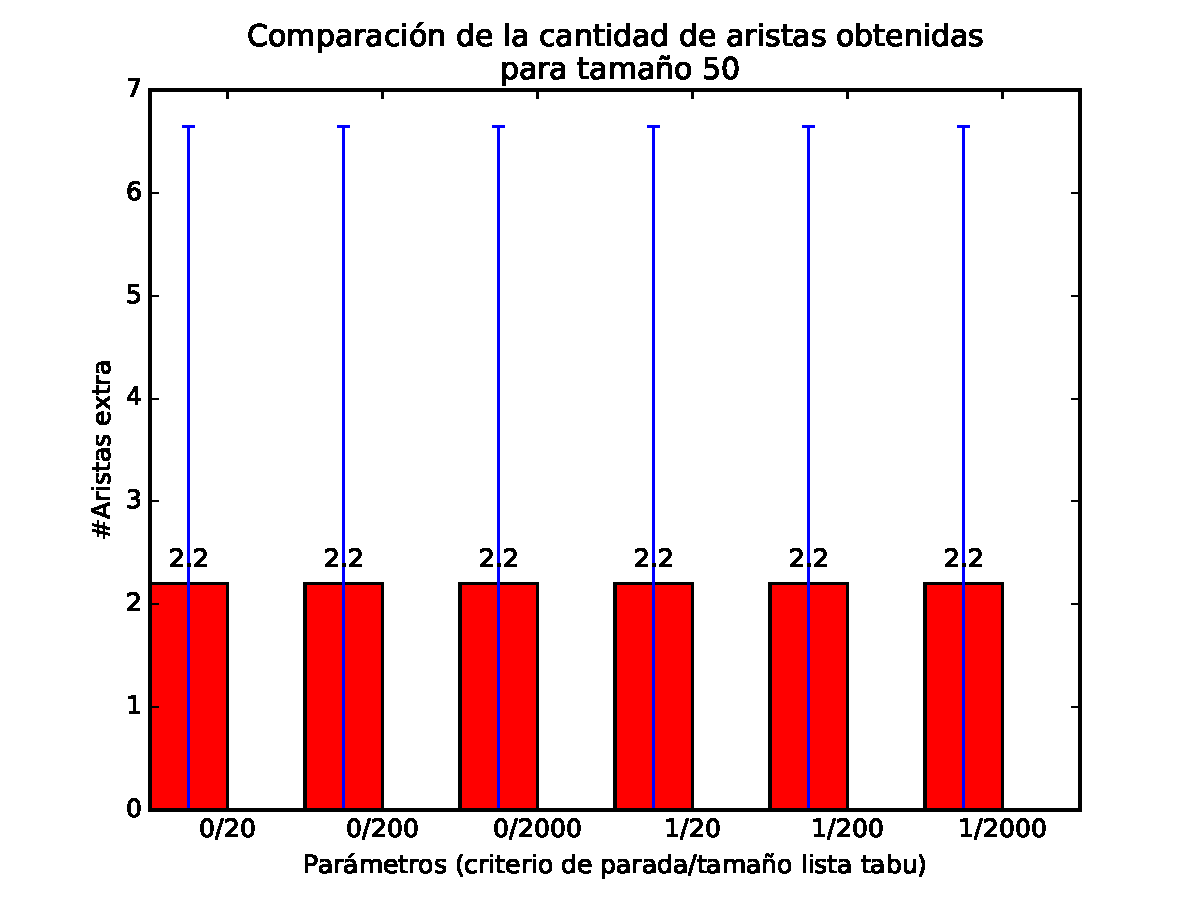
\includegraphics[width=0.8\textwidth]{graficos/problema_6/calidad0.pdf}
	\caption{}
	\label{fig:problema6-calidad0}
\end{figure}


\begin{figure}[H]
 \centering
	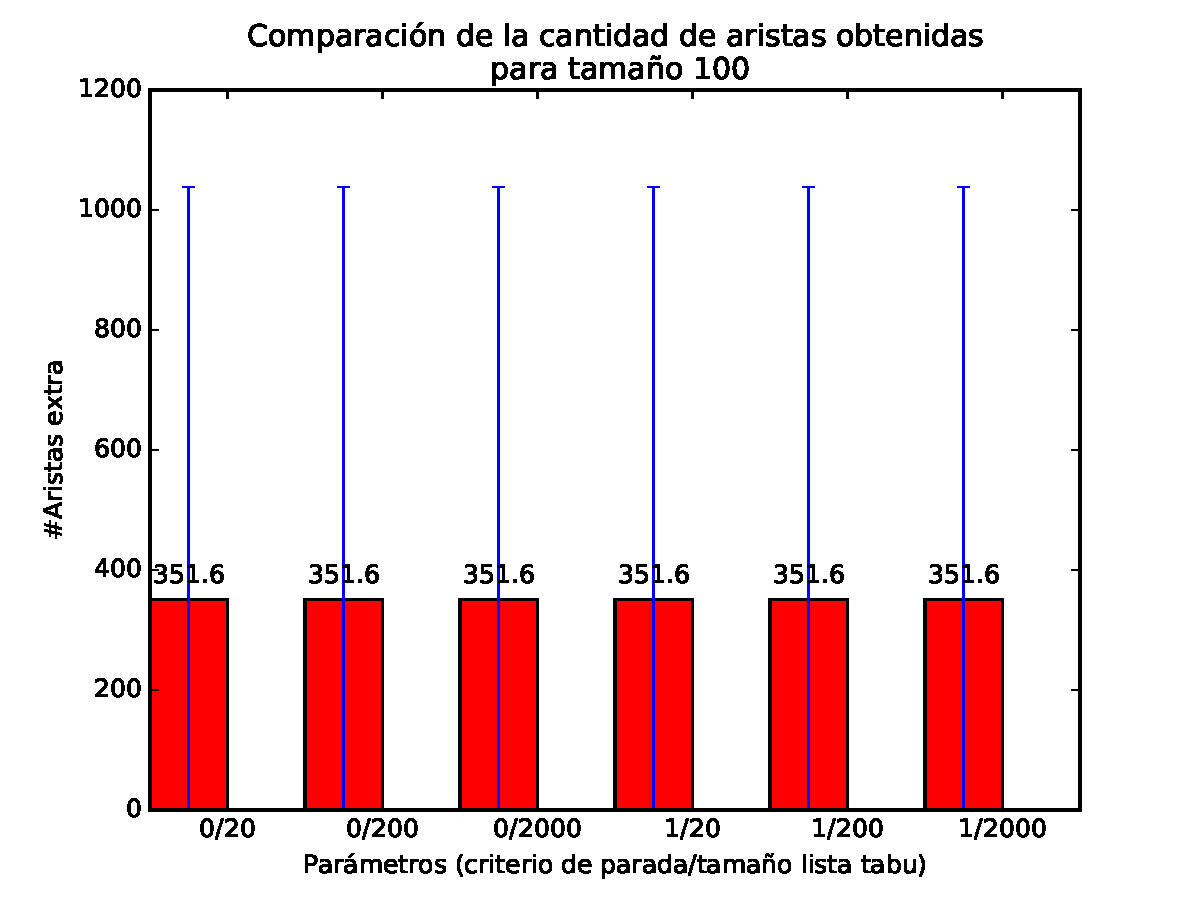
\includegraphics[width=0.8\textwidth]{graficos/problema_6/calidad1.pdf}
	\caption{}
	\label{fig:problema6-calidad1}
\end{figure}

\begin{figure}[H]
 \centering
	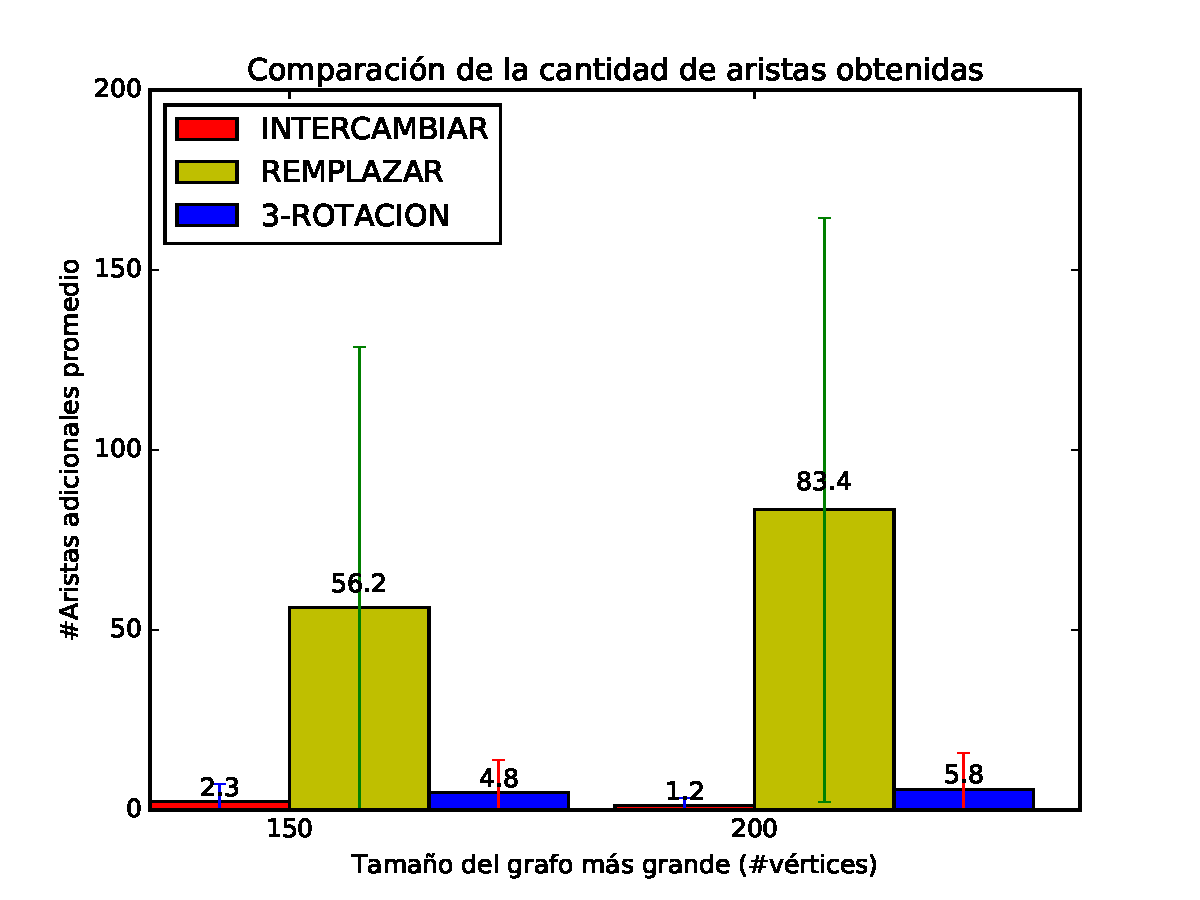
\includegraphics[width=0.8\textwidth]{graficos/problema_6/calidad2.pdf}
	\caption{}
	\label{fig:problema6-calidad2}
\end{figure}

En los gráficos se marca el promedio con una barra y la desviación estándar con un segmento.

Como podemos observar, no hay diferencia en el promedio de calidad de las mediciones.
Sin embargo, pudimos observar algunas diferencias en los máximos y los mínimos. Los mínimos de la variante que cuenta cuantas iteraciones no se mejoró eran mas altos.

Esto se debe a que el tamaño de los grafos no es lo suficientemente grande como para que dos algoritmos buenos hagan diferencia. Sin embargo, los grafos son lo suficientemente grandes como para asegurarnos que la diferencia entre las variantes no será demasiada en ningún caso (salvo casos patológicos).


A continuación, analizaremos los tiempos de los algoritmos. Nuestra expectativa, es que el tiempo que tarda la variante 0, es decir, la que fija la cantidad de iteraciones máxima sin que se mejore la solucion, va a ser mejor dado que optimiza la cantidad de iteraciones "ociosas", sobre todo en grafos chicos, donde la búsqueda se estanca relativamente rápido.

Además, esperamos que las variantes que tienen una lista tabú más larga tardan más, debido a que usamos una lista enlazada (std::list) para representarla, por lo que la búsqueda dentro de ella tiene complejidad lineal.

%% TIEMPOS
\begin{figure}[H]
 \centering
	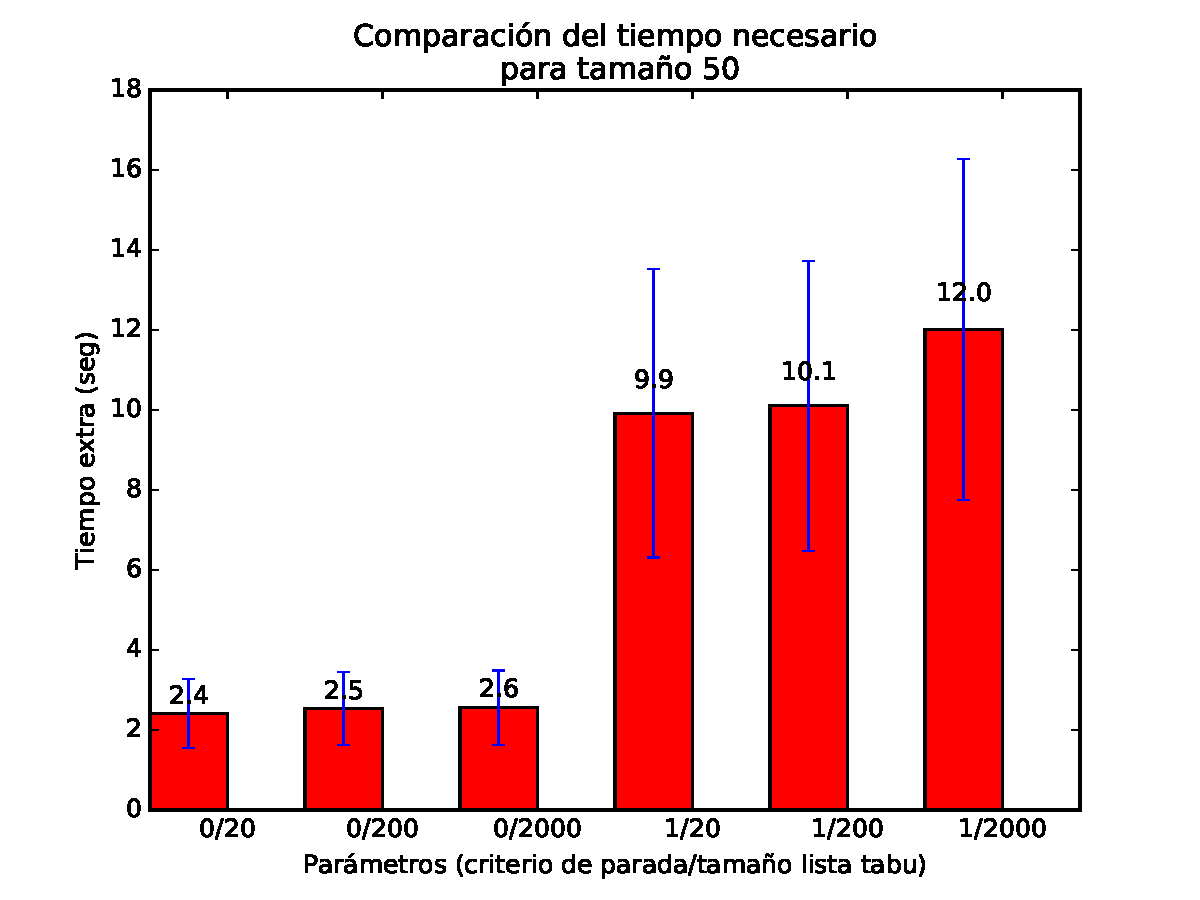
\includegraphics[width=0.8\textwidth]{graficos/problema_6/tiempo0.pdf}
	\caption{}
	\label{fig:problema6-tiempo0}
\end{figure}

\begin{figure}[H]
 \centering
	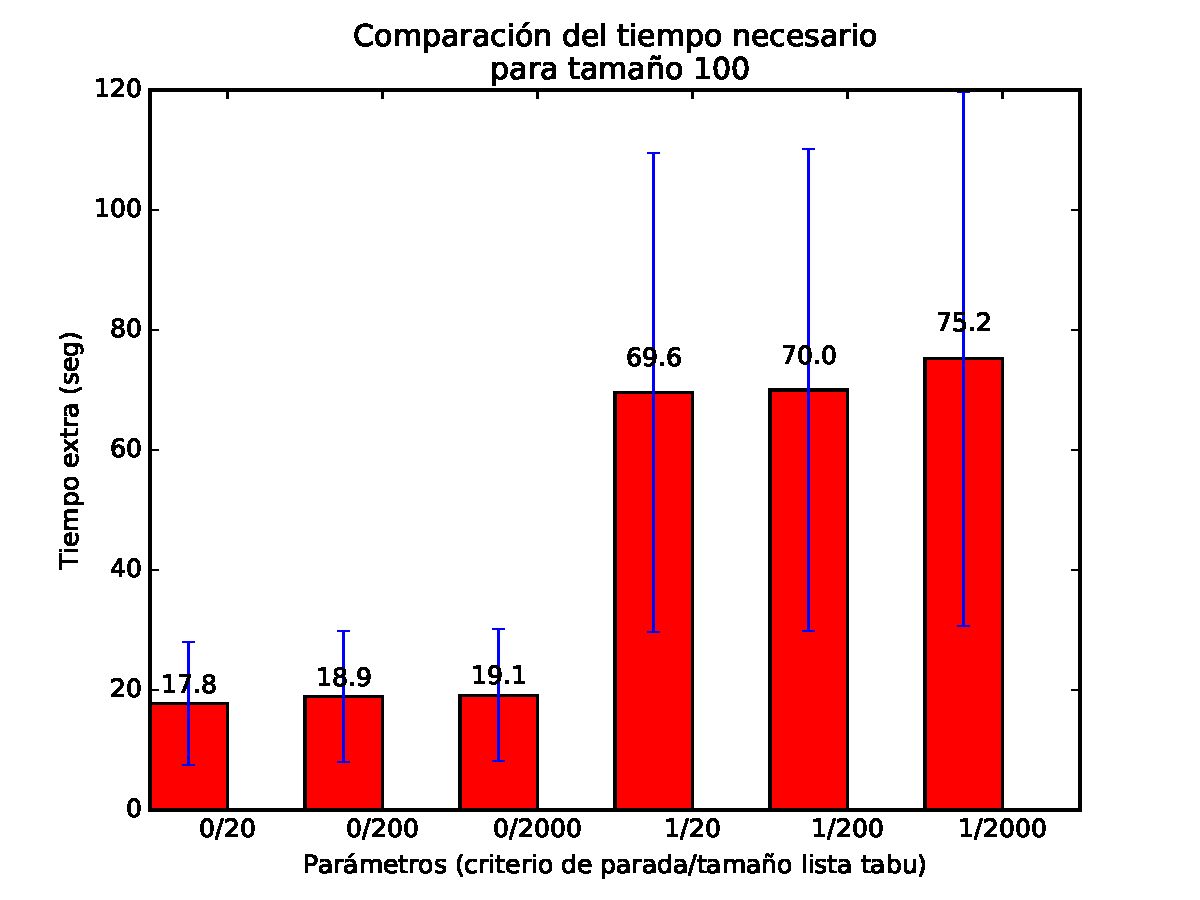
\includegraphics[width=0.8\textwidth]{graficos/problema_6/tiempo1.pdf}
	\caption{}
	\label{fig:problema6-tiempo1}
\end{figure}

\begin{figure}[H]
 \centering
	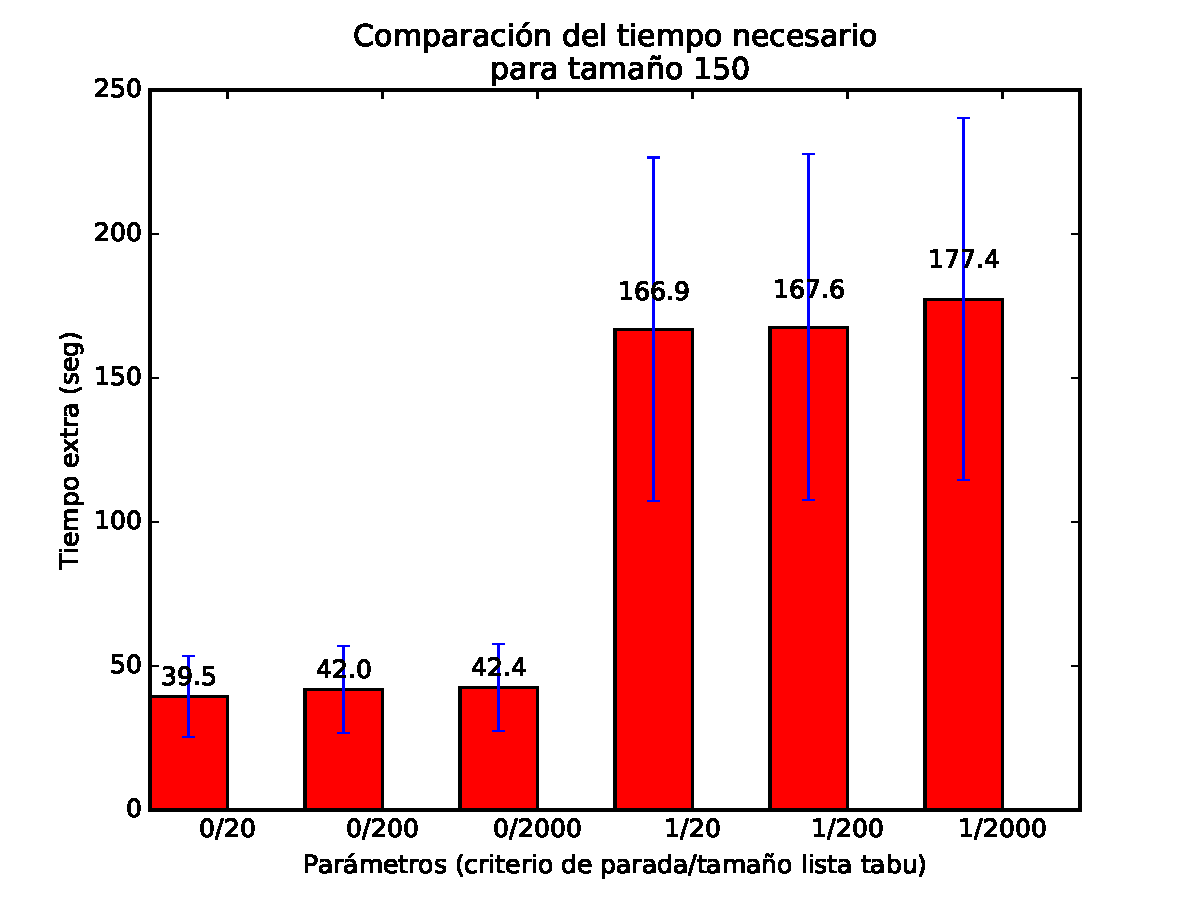
\includegraphics[width=0.8\textwidth]{graficos/problema_6/tiempo2.pdf}
	\caption{}
	\label{fig:problema6-tiempo2}
\end{figure}

En los gráficos se observa que confirmamos nuestras teorias de una manera bastante sólida.

Esto nos permite concluir que, aunque la calidad de las variantes es realmente similar, el tiempo que tardan los algoritmos es distinto, lo que nos permite concluir que la relación costo calidad de los algoritmos sí es diferente..

Esta relación costo calidad puede verse en los gráficos siguientes. En estos gráficos, dividimos la cantidad de aristas extra, sobre la el tiempo que tarda el algoritmo. Es decir, a más alto, mejor es el algoritmo.



%% COCIENTE

\begin{figure}[H]
 \centering
	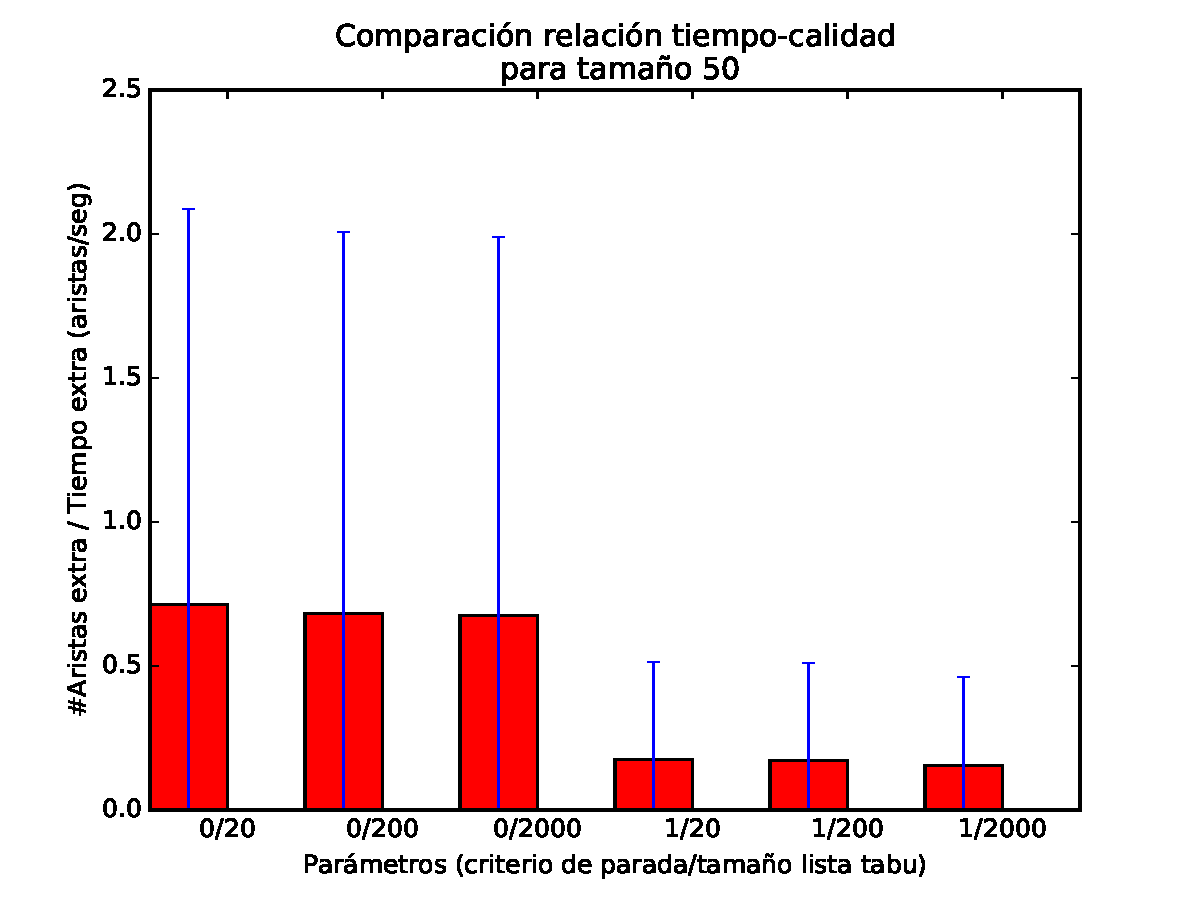
\includegraphics[width=0.8\textwidth]{graficos/problema_6/cociente0.pdf}
	\caption{}
	\label{fig:problema6-cociente0}
\end{figure}

\begin{figure}[H]
 \centering
	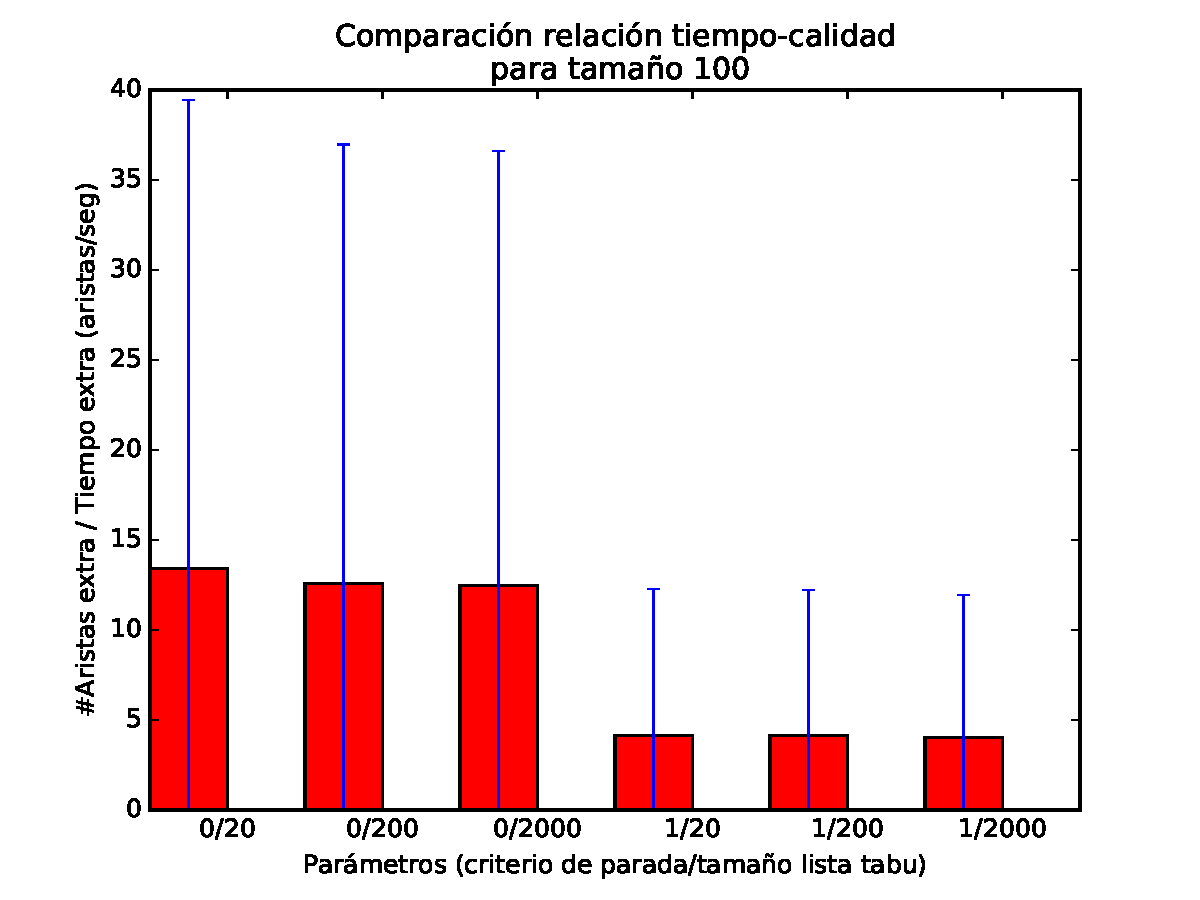
\includegraphics[width=0.8\textwidth]{graficos/problema_6/cociente1.pdf}
	\caption{}
	\label{fig:problema6-cociente1}
\end{figure}

\begin{figure}[H]
 \centering
	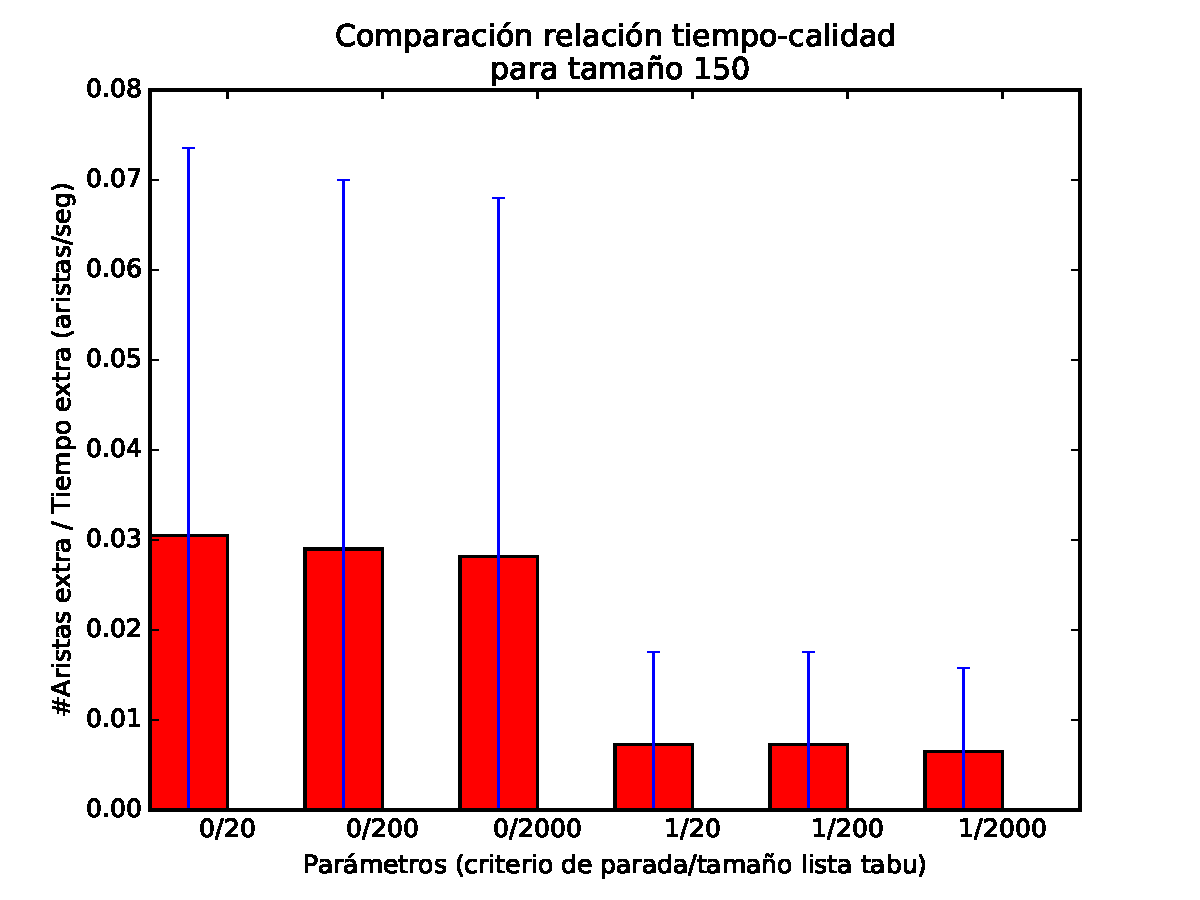
\includegraphics[width=0.8\textwidth]{graficos/problema_6/cociente2.pdf}
	\caption{}
	\label{fig:problema6-cociente2}
\end{figure}


